\documentclass[a4paper]{article}
\usepackage{hyperref}
\usepackage{graphicx}
\usepackage{caption}
\usepackage{subcaption}
\usepackage{listings}
\usepackage{algorithm}
\usepackage{algpseudocode}
\graphicspath{ {./images/} }

\usepackage{xcolor}

\definecolor{codegreen}{rgb}{0,0.6,0}
\definecolor{codegray}{rgb}{0.5,0.5,0.5}
\definecolor{codepurple}{rgb}{0.58,0,0.82}
\definecolor{backcolour}{rgb}{0.95,0.95,0.92}

\lstdefinestyle{mystyle}{
    backgroundcolor=\color{backcolour},   
    commentstyle=\color{codegreen},
    keywordstyle=\color{magenta},
    numberstyle=\tiny\color{codegray},
    stringstyle=\color{codepurple},
    basicstyle=\ttfamily\footnotesize,
    breakatwhitespace=false,         
    breaklines=true,                 
    captionpos=b,                    
    keepspaces=true, 
    language=Python,               
    numbers=left,                    
    numbersep=5pt,                  
    showspaces=false,                
    showstringspaces=false,
    showtabs=false,                  
    tabsize=2
}

\lstset{style=mystyle}

\title{SON implementation with Spark in Python}
\author{Carli Alberto VR473845\and Fraccaroli Leonardo VR474539}
\date{}

\begin{document}
	\maketitle
	\tableofcontents
	\newpage
	\section{Introduction}
	Finding frequent itemsets is frequently done in data mining domains to understand which items frequently appear together. The definition of ``items'' is beyond the scope of this work. Suffice to say that we treated them as binary variables, listed in a basket only when their value is True. In our project a \textbf{basket} is a list of items that appear together (for example products bought by a customer).
	
	This is an analysis that can be performed on almost any dataset, but is especially suited for domains like e-commerce. It is an interesting challenge to try and take the system to the extreme where the dataset is so large that it does not fit on any single machine's memory and it is more convenient to distribute analysis to multiple compute units.
	
	We tried to imagine ourselves into a big e-commerce company that stores transaction data on a distributed database and wants to periodically analyse data to understand which items are usually bought together. \\
	The data is simply a list of items bought at any time. To store the data in a distributed database we used MongoDB and thus we needed a version of parallel \textbf{Apriori} (an algorithm to find frequent itemsets on a single machine). \\
	We parallelized Apriori by using Spark in Python and using the \textbf{SON} algorithm as proposed in chapter 6.4.4 of the \href{http://www.mmds.org/}{Mining Massive Datasets} book.
	\newpage

	\section{SON}
	In this section we will dissect our implementation of SON through Spark, describing all the steps of computation and their result.
	
	\subsection{SON Algorithm}	
	The algorithm, as described in the book, involves two phases of MapReduce as follows:
	\begin{enumerate}
	\item The \textit{mapper} basically executes Apriori (or any other algorithm to find frequent itemsets) on every batch of baskets, extracting all frequent itemsets for each batch. The required frequency (support) is reduced by a factor equal to the number of batches the data is partitioned in, using the following formula:
	\[ batch\_support = basket\_size / total\_data\_size * total\_support \]
	The \textit{reducer} combines all the frequent itemsets from every batch in a single list. These are \textit{candidate frequent itemsets}.\\
	This step removes false negatives by keeping all the itemsets that are frequent in at least one batch.
	\item The \textit{mapper} takes a batch of the data and counts the occurrences of every candidate itemset.\\
	The \textit{reducer} adds up the counts from every batch and finally filters out the infrequent ones using the original support.\\
	This step removes false positives by keeping only the itemsets that are globally supported.
	\end{enumerate}
	The result of these phases is the list of \textit{frequent itemsets}.
	
	\subsection{Our Implementation}
	Our implementation expects a $pyspark$ RDD. We will discuss our first implementation, following the steps as described in the book, and then we will show our second implementation, 
	which is a bit different and cuts around some corners that we found out to be unnecessary in Spark. These changes help improving the overall performance.
	
	\subsubsection{First Map}
	The input data is in the form of a list of lists, where every internal list holds a set of strings, which are the items.
	We performed a map operation to transform the data into a list of sets, where every set is a basket (fig.\ref{fig:input_data}). 
	This is done with the $map$ function of $pyspark$:
	\begin{lstlisting}
.map(set)
\end{lstlisting}
	
	Apriori algorithm is applied to every batch, which returns a list of frequent itemsets (fig.\ref{fig:apriori}). This is done with the $mapPartitions$ function of $pyspark$: 
\begin{lstlisting}
.mapPartitions(lambda x: apriori(list(i for i in x), support, data_size))
\end{lstlisting}
	where \texttt{x} is a batch, \texttt{support} is the support for the entire dataset and \texttt{data\_size} is the total number of baskets in the entire dataset (they are needed in \texttt{apriori()} to calculate the batch support).
	\texttt{x} is an \textit{itertools.chain} object, so we needed to convert it to a list. After some testing we found out that the fastest way is to use a generator object instead of the $list()$ constructor.\\
	We will discuss our implementation of Apriori, in details, in section \ref{section:apriori}. We chose not to keep only the frequent supersets because we saw that there may be cases where the larger set is not globally supported, but the smaller ones are.\\
	Then every itemset is ``emitted'' with a 1, to facilitate the reduce phase:
\begin{lstlisting}
.map(lambda x: (x, 1))
\end{lstlisting}
	
	\subsubsection{First Reduce}
	Now the result of the previous step is grouped by key (fig.\ref{fig:grouped}) and the list of counts discarded entirely:
	\begin{lstlisting}
.groupByKey()
.map(lambda x: x[0])
\end{lstlisting}
	The result is the list of all itemsets that appear at least once (fig.\ref{fig:candidate_fi}), which means that they are frequent in at least one batch.\\
	Then the list is collected and broadcasted to all the nodes.
	
	\begin{figure}[h]
		\centering
		
		\begin{subfigure}[b]{0.24\textwidth}
			\centering
			\includegraphics[width=\textwidth]{Baskets.PNG}
         	\caption{Input data}
         	\label{fig:input_data}
		\end{subfigure}
		\hfill
		\begin{subfigure}[b]{0.24\textwidth}
			\centering
			\includegraphics[width=\textwidth]{Batch_fi.PNG}
         	\caption{Apriori on batch}
         	\label{fig:apriori}
		\end{subfigure}
		\hfill
		\begin{subfigure}[b]{0.24\textwidth}
			\centering
			\includegraphics[width=\textwidth]{grouped.PNG}
         	\caption{First reduce}
         	\label{fig:grouped}
		\end{subfigure}
		\hfill
		\begin{subfigure}[b]{0.24\textwidth}
			\centering
			\includegraphics[width=\textwidth]{candidates.PNG}
         	\caption{Candidate frequent itemsets}
         	\label{fig:candidate_fi}
		\end{subfigure}
	\caption{Results of first MapReduce phase}
	\end{figure}
	
	\subsubsection{Second Map}
	Now we need to count the occurrences of every itemset in the whole dataset.\\
	We do it on every partition:
	\begin{lstlisting}
.mapPartitions(lambda x: count_frequencies(candidate_frequent_itemsets.value, list(i for i in x)))
\end{lstlisting}
	The result is a list of tuples where the first element is the itemset and the second is the number of occurrences of that itemset in the partition (fig.\ref{fig:counts}).
	
	\subsubsection{Second Reduce}
	Now the itemsets are reduced across partitions by summing counts (fig.\ref{fig:totals}) and then filtered based on the global support:
	\begin{lstlisting}
.reduceByKey(lambda x, y: x + y)
.filter(lambda x: x[1] / data_size >= support)
\end{lstlisting}
	The result is the list of every itemset which is supported enough to be considered frequent.
	
	\begin{figure}[h]
		\centering
		
		\begin{subfigure}[b]{0.4\textwidth}
			\centering
			\includegraphics[width=\textwidth]{counts.PNG}
         	\caption{Counts of itemsets for every batch}
         	\label{fig:counts}
		\end{subfigure}
		\hfill
		\begin{subfigure}[b]{0.4\textwidth}
			\centering
			\includegraphics[width=\textwidth]{totals.PNG}
         	\caption{Sum of counts across partitions}
         	\label{fig:totals}
		\end{subfigure}
	\end{figure}
	
	
	\subsubsection{Other considerations and final implementation of SON}
	Initially, we implemented the code following the instructions on the book using Spark operations, but then we found another method that has slightly better performances to implement the first
	pass of MapReduce.\\
	So the final implementation went from
	\begin{lstlisting}
candidate_frequent_itemsets = (baskets
    .mapPartitions(lambda x: apriori(list(i for i in x), support, data_size))
    .map(lambda x: (x, 1))                                             
    .groupByKey()                                                      
    .map(lambda x: x[0])                                               
    ).collect()
\end{lstlisting}
to
	\begin{lstlisting}
candidate_frequent_itemsets = (baskets
    .mapPartitions(lambda x: apriori(list(i for i in x), support, data_size))
    ).collect()
candidate_frequent_itemsets = list(set(candidate_frequent_itemsets))
\end{lstlisting}
followed by the broadcast of the variable to all nodes
\begin{lstlisting}
	candidate_frequent_itemsets = baskets.context.broadcast(candidate_frequent_itemsets)
\end{lstlisting}
	
	The second MapReduce pass is the same as before, because we didn't manage to identify unnecessary steps.

	\newpage
	
	\section{Apriori}
	\label{section:apriori}
	
	Apriori is the most known algorithm to find frequent itemsets in a dataset. The algorithm relies on the monotonicity of support, by building candidates from smaller sets which are knowingly frequent. 
	This is because it is impossible for an itemset to be frequent if every item it is composed of is not frequent by itself. The algorithm \ref{algo:apriori} shows the Apriori pseudocode.
	
	To benchmark SON execution we compared it to an implementation of Apriori, which we made ourselves (\textit{Scripts/apriori.py}).
	
\begin{algorithm}
\caption{Apriori pseudocode}
\label{algo:apriori}
\begin{algorithmic}[1]
\Function{apriori}{data, total\_support, total\_db\_size}
	\State $L_1 \gets \{frequent \ 1-itemsets\}$ \Comment{\textcolor{gray}{\emph{\parbox[t]{.3\linewidth}{$L_k$ is the set of truly frequent itemsets of size $k$}}}}
    	\State $k \gets 2$
    	\While{$L_{k-1}$ is not empty}
    		\State create $C_k$ using $L_{k-1}$ (by adding singlets) \Comment{\textcolor{gray}{\emph{\parbox[t]{.3\linewidth}{$C_k$ is the set of candidate itemsets of size $k$}}}}
    		\State count occurrences of each itemset of $C_k$ in $data$
    		\State filter out non-frequent itemsets in $C_k$
    		\State $L_k \gets C_k$
    		\State $k \gets k+1$
    	\EndWhile
\EndFunction
\end{algorithmic}
\end{algorithm}

    In our implementation of the Apriori pseudocode we first extract the items from the data, keep the frequent ones and then use them to build all the candidate couples.
	Then we count them, filter out infrequent ones and then expand those couples to form triples and so on.\\
    We also added a fail-safe feature to our implementation: if the support in a partition is so low that all possible itemsets are frequent, it doesn't even begin to create them. It instead prints 
	some error message and returns None.\\
	The other threads won't stop for this, but detecting at least one null result will void all other results (we will discuss more on this in section \ref{section:conclusion}).

    Moreover, we found a state-of-the-art implementation of Apriori: it is called \href{https://github.com/tommyod/Efficient-Apriori}{Efficient Apriori}, and it is the fastest implementation of Apriori. 
	We tried to use it in our SON code and we can appreciate the improvements in execution time in fig.\ref{fig:aprioribenchmark-h} and fig.\ref{fig:aprioribenchmark-e}, which will be further discussed in section \ref{section:results}. 
	
	\section{Benchmark}
	We have run some benchmarks to better understand how SON compares to Apriori.
	
	In order to do so we made a script for the specific purpose of being able to programmatically change parameters and subsample datasets.
	Also, we implemented a grid search to test many parameters. We also added a logging feature to our project to better follow executions and ease debug.
	
	We compared our implementations, both \textbf{based on DB} (using the \href{https://www.mongodb.com/docs/spark-connector/current/}{MongoDB Connector for Spark}, which is kind of a ``real world'' example, see section \ref{section:database})
	and \textbf{in memory} (having all the data locally), to the method $FreqItems$, provided by $pyspark.sql$. 
	This function implements the algorithm proposed by \href{https://doi.org/10.1145/762471.762473}{Karp, Shenker, and Papadimitriou}, which uses a modified version of FP-Tree to be more parallelizeable. 
	This function proved itself to be absurdly fast, at the expense of false positives.
	Both a  ``simple'' dataset and a ``harder'' one were used to compare performances.

	\subsection{Datasets}
	The first ``easier'' dataset is from UCI \href{https://archive.ics.uci.edu/ml/datasets/Travel+Reviews#}{(Travel Reviews)} and is composed of averages of scores that every user gave to some
	categories of places on TripAdvisor. We expanded it with some random data to have a bigger dataset ($\sim$3 million of rows) and we arbitrarily kept only the ones with an average mark above 2.5. This way our dataset is in the form:
	\[ user\_id: category1, category2, \ldots \]
	It is considered ``easy'' because it is very sparse and the number of items is very low (10 items).

	The second ``harder'' dataset is a collection of transactions where some users bought some items in a transaction, again from UCI \href{https://archive.ics.uci.edu/ml/datasets/online+retail}{(Online Retail)}.
	We decided to form transactions on invoices, so we extracted the list of items bought together.
	This way our dataset is in the form:
	\[ invoice\_no: item\_code1, item\_code2, \ldots \]
	It is considered ``harder'' because of the higher number of items (4059) and the large variability in basket size.

	Since the most part of the algorithm consists in counting frequencies of itemsets in the dataset, we tried to optimize time a little bit, by converting the baskets of items from a list of lists to
	a list of sets. This way every \texttt{itemset in basket} operation in Python takes constant time instead of linear.\\

	\subsection{Database}
	\label{section:database}
	Part of our project was to explore how Spark interacts with a database (we used MongoDB).
	
	We found that there is a \href{https://www.mongodb.com/docs/spark-connector/current/}{MongoDB Connector for Spark} to connect to a MongoDB database and read the data from it as well as write the results back to it.
	
	The main difference between a local spark instance (i.e. reading from local memory and not from a database) is that the environment is a $SparkSession$ (instead of a $SparkContext$), which allows to use connectors 
	to read and write data from databases as well as repartition it.

	A $partitioner$ can be specified to regulate how the data is handled and to change how it is distributed by providing the abstraction layer to work on a database like an RDD. 
	The partitioner attempts to distribute access load across the database and can be configured to adapt to the unique requirements of each individual database. For instance the default partitioner is a $SamplePartitioner$ (the one we decided to use), which
	distributes the data based on pages count up to a maximum partition size, then there is the $PaginateBySizePartitioner$ which creates partitions of specified weight and $PaginateIntoPartitionsPartitioner$
	which creates the required number of partitions, regardless of their weights.

	The read data is in the form of a $DataFrame$. The main difficulty when using a $DataFrame$ is that the underlying data is represented as rows, with specific access methods. Despite that, it appears 
	to be a wrapper of an RDD which allows to even use SQL queries on the data. It is still possible to extract the RDD and use it directly. That's what we did: we used the $DataFrame$ to read data from a database, but then extracted the RDD and used the commonly known methods to perform the actual computation to avoid struggling around
	the $DataFrame$.

	We tried executing SON on a sharded database. Spark makes it transparent to the user, because the connector simply connects to the database master node and it is the database that handles the
	connection to the shards. On the other side, the setup of the sharded database is not trivial.\\
	After the connection, Spark provides a specific partitioner, the \textit{ShardedPartitioner} which theoretically creates a partition per shard and assigns it to the same machine, to maximize data locality.

	We tried this configuration and although it is theoretically better for load distribution and allows exploiting data locality, it was difficult to setup the database sharding, it added complexity 
	in handling and distributing data while not providing any performance improvement. 
	In fact, working on a single machine it was impossible to properly test performances and although we didn't notice difference in execution time, we couldn't determine if that was because of our 
	setup or configuration mistakes.
	
	Considered all these problems, we settled on a single node database with a default partitioner.


	\subsection{Results}
	\label{section:results}
	% Setups (CPU, MEMORY, MONGO)
	After some testing we figured that both the support and the partitions count played a major role in execution time, on top of the dataset. We tested a mix of different supports on each dataset with the growth of both dataset size and partition number.

	These tests were performed on a 6 core $i5-8600 @3.10GHz$, with 16 GB DDR4 memory $@2666Mhz$, but the driver was capped at 4GB and executors were capped at 2GB RAM.
	
	We made different tests considering both a minimum support and a reasonable support:
	\begin{enumerate}
		\item \textbf{Minimum support} required to produce frequent itemsets. In the case of our datasets, after some testing we figured that this is 0.3 for the ``easy'' dataset and 0.1 for the ``hard'' one.\\
		We tested execution time as the dataset grows with 1 (fig.\ref{fig:1par-minsup}) and 2 (fig.\ref{fig:2par-minsup}) partitions.
		\item \textbf{Reasonable support} that is more likely used in a real scenario. Here we tried to see how performance varied increasing the number of partitions, using the whole datasets.\\
		We tested with support 0.75 (fig.\ref{fig:075sup}) and 0.9 (fig.\ref{fig:09sup}).
	\end{enumerate}

	We performed all these tests with our implementation of Apriori, to show how its execution time compares to the SON one.
	
	We noticed the overhead added by the second MapReduce phase of SON using a single partition when the number of baskets is high (e.g. easy dataset), compared to Apriori. For example in figure \ref{fig:1par-minsup-a} we can see the overhead of the second MapReduce phase is much bigger than in the figure \ref{fig:1par-minsup-b}, because of the bigger size of the dataset. This is especially visible when using efficient-apriori because the time spent in the first MapReduce phase is negligible compared to the second one (fig.\ref{fig:aprioribenchmark-e}).

	Not all the difference in time is due to the time taken by the second MapReduce phase. Indeed, we found that the \textit{collect()} operation takes a time proportional to the dataset size and it is not
	negligible. In our testing it takes about 4 seconds for the 3 million rows of the easy dataset. This \textit{collect()} time does not depend on pending operations on the collected RDD and it slightly increases with the number of partitions. And this is just on one machine. We expect it to be much
	more significant when using a cluster with network times.

	On the other side, from figure \ref{fig:2par-minsup}, it is evident that the performance of SON improves significantly (compared to Apriori) when handling datasets with a higher number of items. %Conversely, when dealing with datasets with a lower support in each partition, resulting in a higher number of candidate itemsets generated by Apriori, the performance of SON decreases, as observed in figures \ref{fig:1-075sup-1ds-par-h} and \ref{fig:1-09sup-1ds-par-h} for the hard dataset.

	Tests show a clear difference in execution time between the local and database based algorithms (fig.\ref{fig:075sup-e} and fig.\ref{fig:09sup-e}, easy dataset), despite SON being exactly the same. This shows that handling the database brings in additional overhead.
	This is partly because of the additional operations we have to do to strip the data from the $Row$ structure and to convert it to a list of lists, but mostly due to the database access. We also noted that the second phase of MapReduce takes a lot longer, although we weren't able to determine if it was due to the database access or to something else.
	
	The figure \ref{fig:result-example} is an example of a result obtained executing the file \textit{benchmark.py}.
	
	\begin{figure}[h]
			\centering
			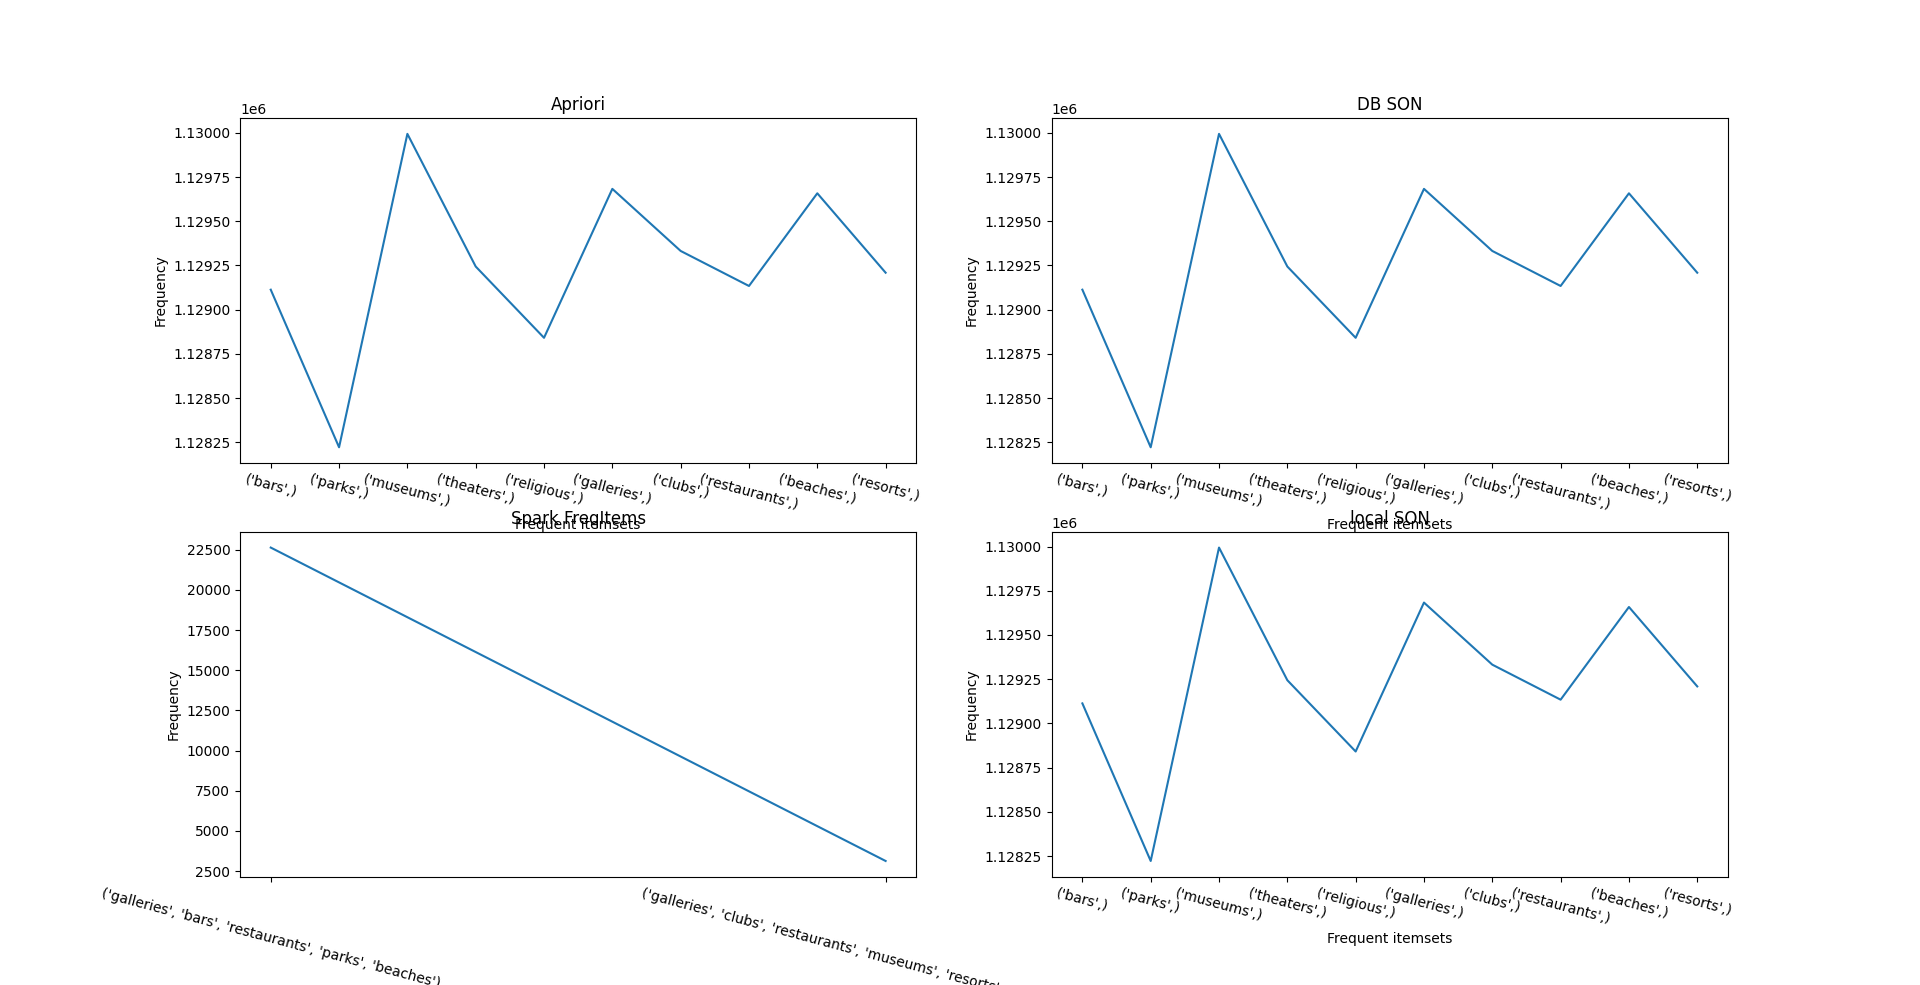
\includegraphics[width=\textwidth]{result_example.png}
         	\caption{Comparison of different algorithms output}
		\label{fig:result-example}
	\end{figure}
	
	\section{Conclusions}
	\label{section:conclusion}
	The main advantage of SON, that we could appreciate in our single machine setup, was the ability to use all the available cores, distributing the load, which could proves highly beneficial to execution time on larger datasets.

	We have seen how easy it is connecting pyspark to a distributed database, eventually sharded.	
	We noticed that the database partitioner optimizes for the database connection (based on the size of the database itself), 
	while the local partitioner ($parallelize$ function) optimizes for exploiting all the resources of the machine.
	
	We have encountered an issue where, in some cases, the scaled support in a partition was so low that a frequency of one (or less) basket was considered frequent, 
	which caused an explosion in the number of candidates generated by Apriori, not because they were actually frequent in the partition, but 
	because every item (and all the combinations in each basket) always appear at least once. 

	In general, the huge reduction in support is an issue that happens every time the global support is too low or when the support is divided over many partitions ($\leq$ 5\% in a single partition).\\
	This is an issue because the core is still Apriori and it's very important that the minimum support is high enough to prune the data as the algorithm works.

	We also noticed that the execution time of the second pass of MapReduce scales a lot with the number of baskets, which has to be considered when deciding how to partition the data.

	Throughout the project, we have come to the understanding that using a distributed algorithm on spark is a balancing act and that even the simplest parameter, like the number of partitions and, consequently how distributable 
	the data is, has to be perfectly balanced and fine tuned while keeping in mind hardware specifics, like the core count, the required support and the characteristics of the dataset to achieve 
	maximum performance.
	

	\newpage
	\appendix 

	\section{Apriori benchmarks}

	\begin{figure}[h]
		\centering
		\begin{subfigure}[b]{0.49\textwidth}
			\centering
			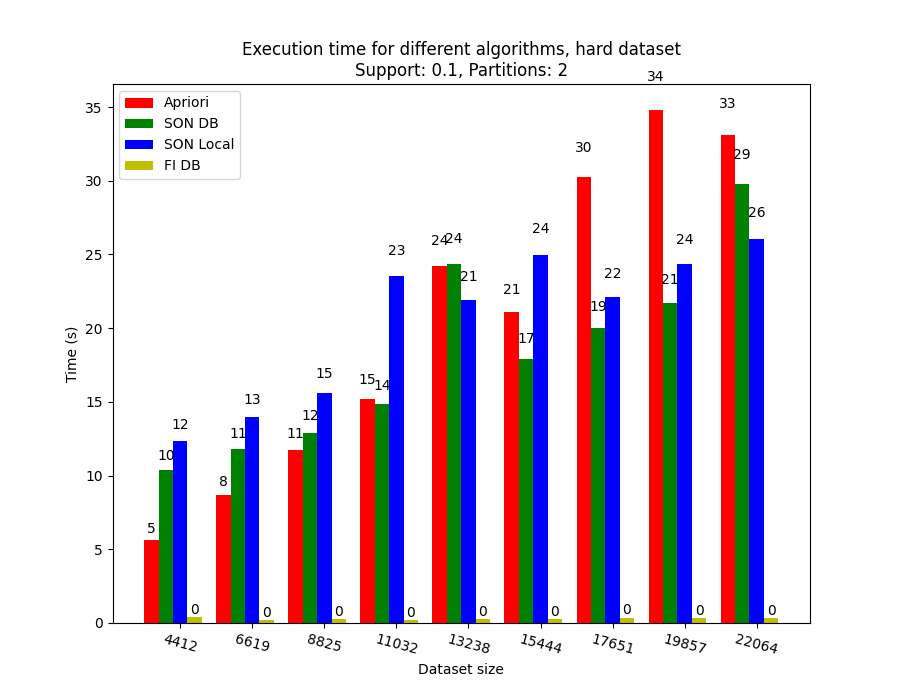
\includegraphics[width=\textwidth]{hard_aprioribenchmark.png}
         	\caption{Apriori}
		\end{subfigure}
		\hfill		
		\begin{subfigure}[b]{0.49\textwidth}
			\centering
			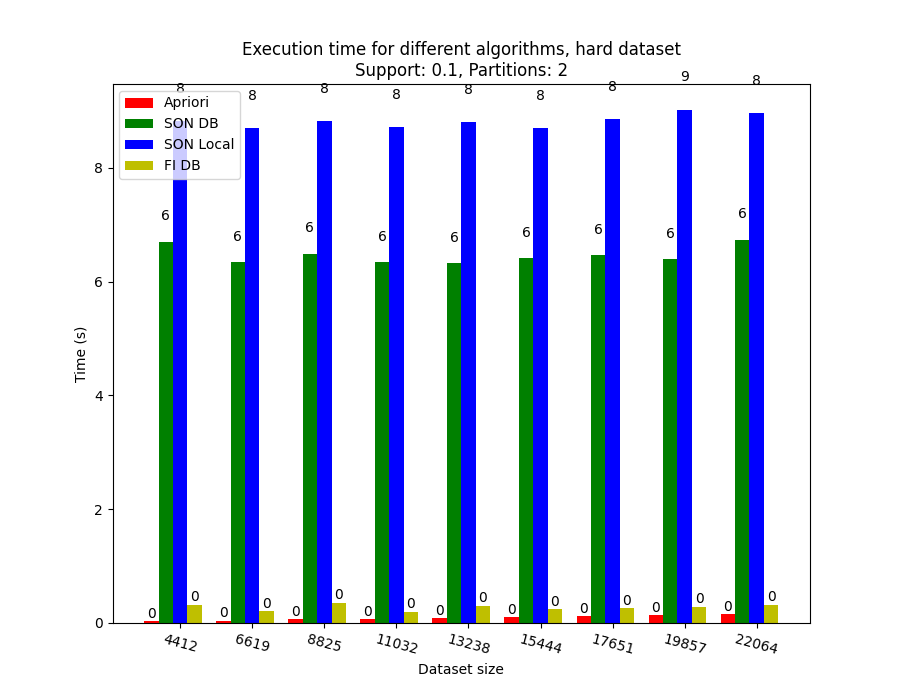
\includegraphics[width=\textwidth]{hard_apriori2benchmark.png}
         	\caption{Efficient-Apriori}
		\end{subfigure}
		\hfill
		\caption{Apriori and Apriori2 (efficient-apriori) benchmark results on the hard dataset}
		\label{fig:aprioribenchmark-h}
	\end{figure}

	\begin{figure}[h]
		\centering
		\begin{subfigure}[b]{0.49\textwidth}
			\centering
			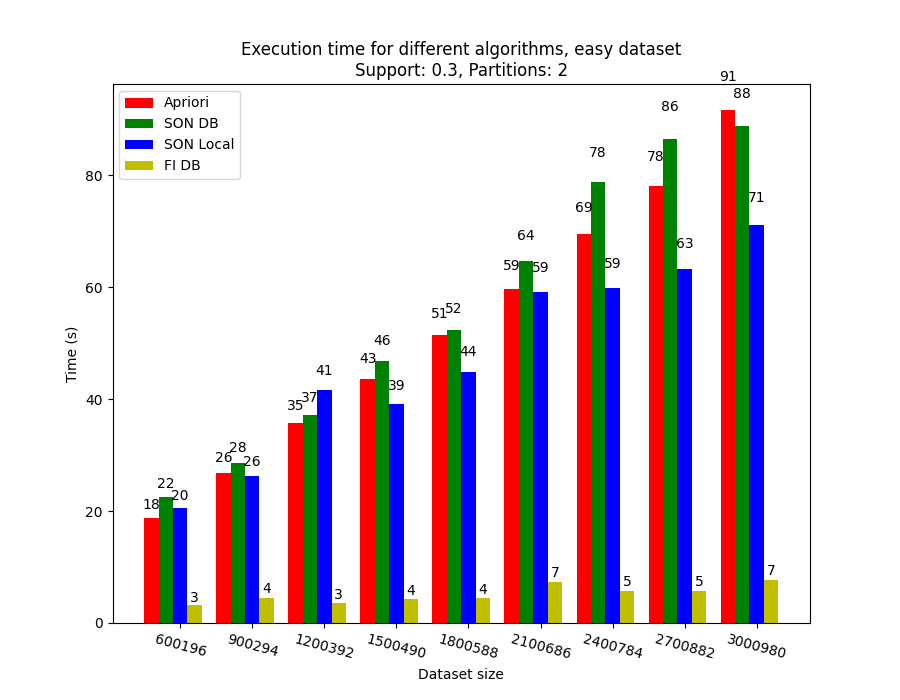
\includegraphics[width=\textwidth]{easy_aprioribenchmark.png}
         	\caption{Apriori}
		\end{subfigure}
		\hfill		
		\begin{subfigure}[b]{0.49\textwidth}
			\centering
			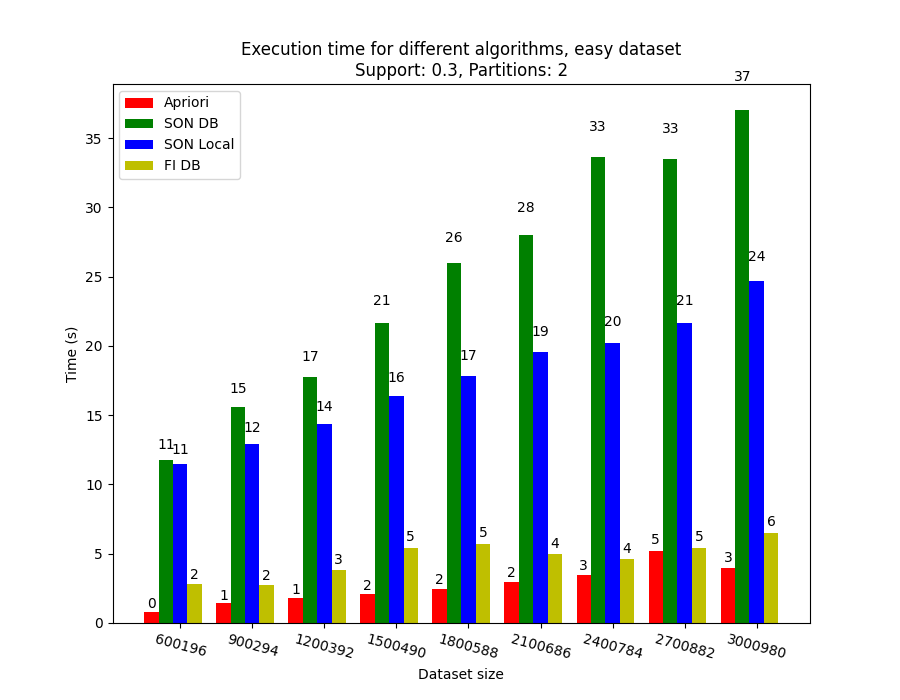
\includegraphics[width=\textwidth]{easy_apriori2benchmark.png}
         	\caption{Efficient-Apriori}
		\end{subfigure}
		\hfill
		\caption{Apriori and Apriori2 (efficient-apriori) benchmark results on the easy dataset}
		\label{fig:aprioribenchmark-e}
	\end{figure}

	\newpage
	\section{Benchmark Images}

	\begin{figure}[h!]
		\centering
		\begin{subfigure}[b]{\textwidth}
			\centering
			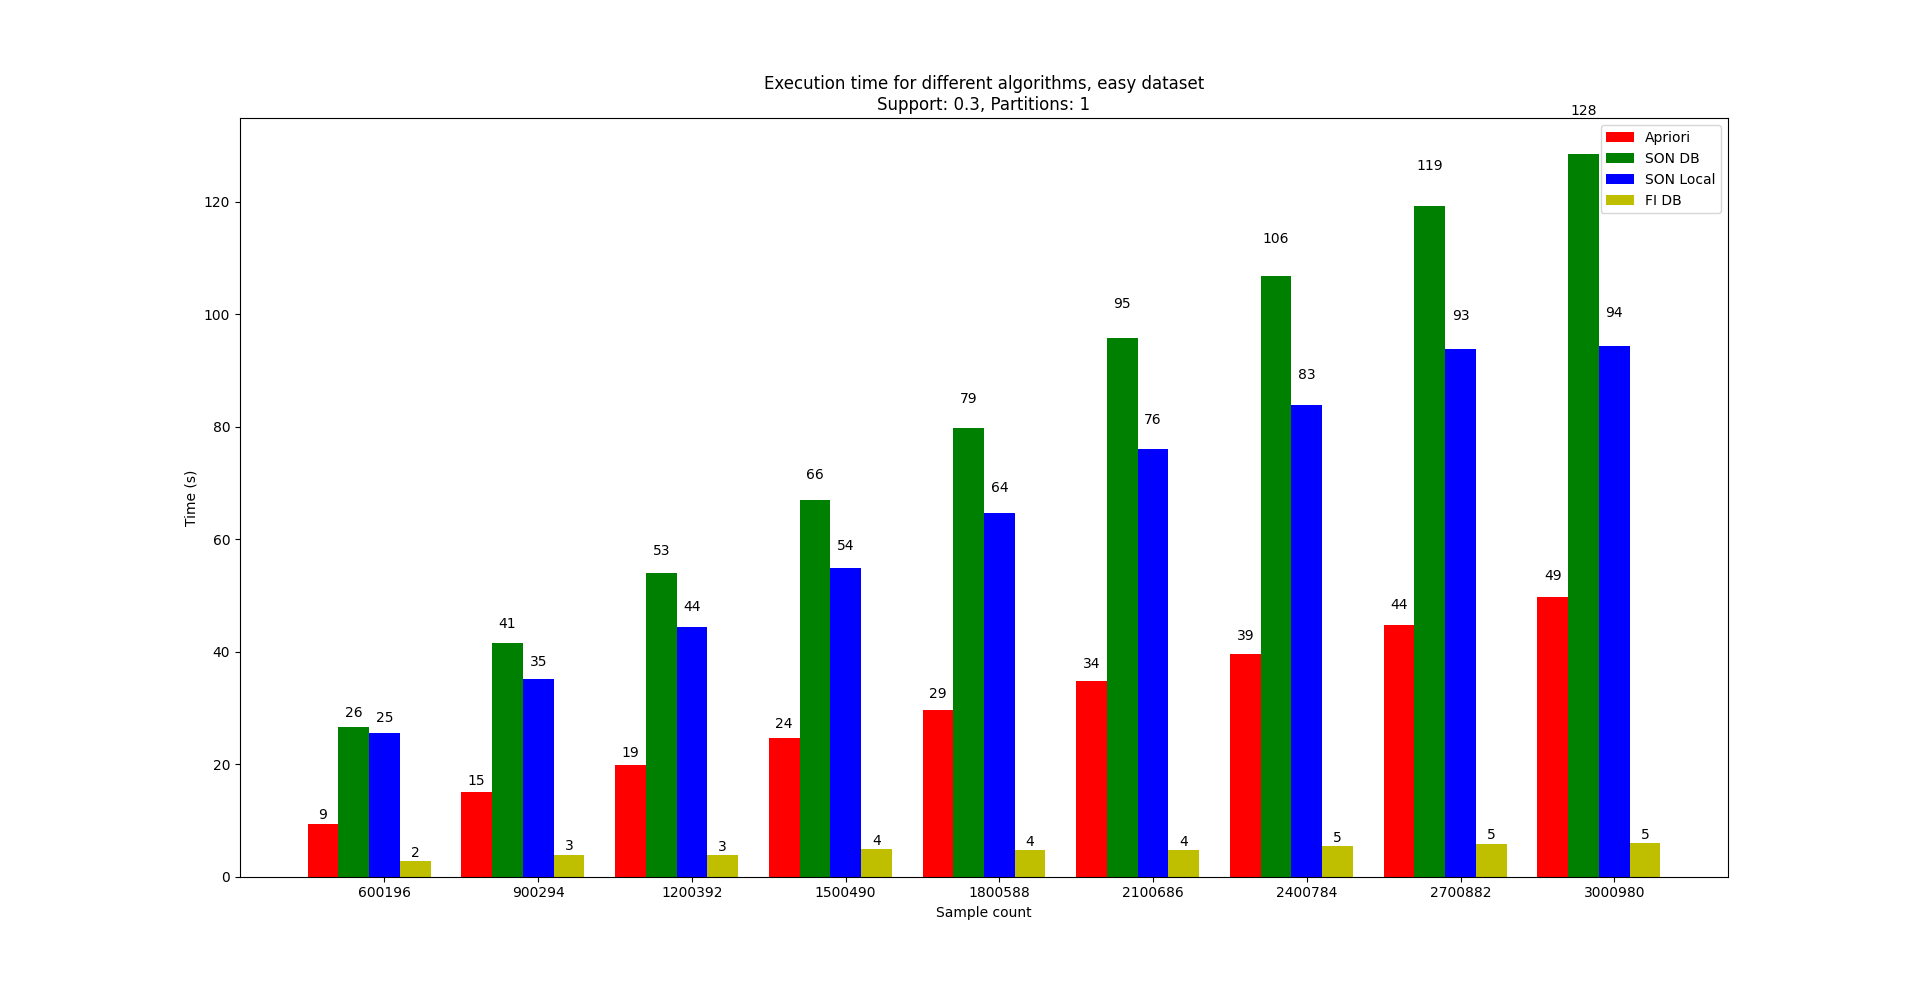
\includegraphics[width=.9\textwidth]{1_easy_0,3_1_dataset.png}
         	\caption{Easy dataset}
         	\label{fig:1par-minsup-a}
		\end{subfigure}
		\begin{subfigure}[b]{\textwidth}
			\centering
			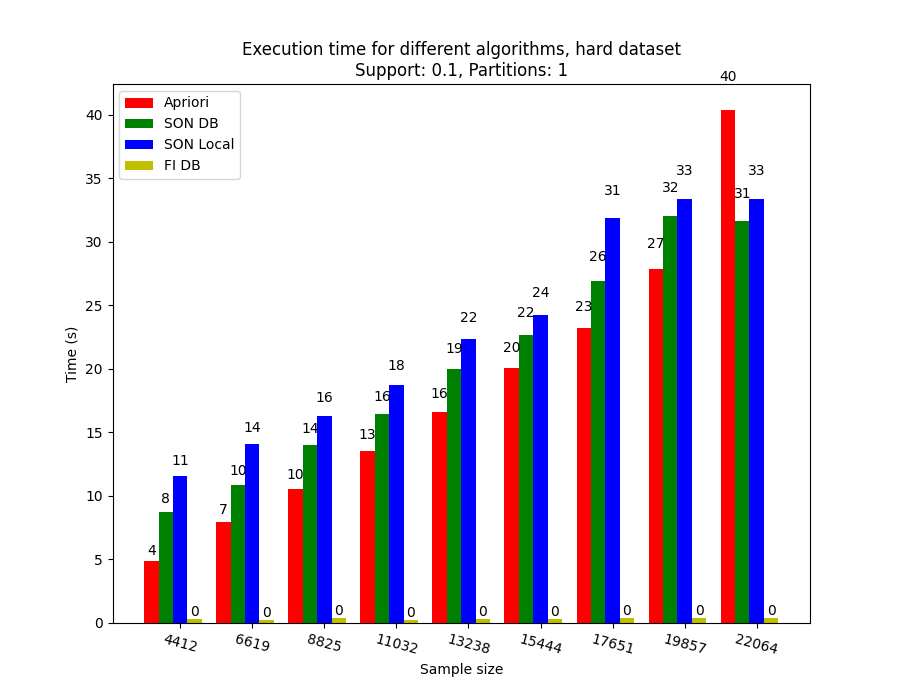
\includegraphics[width=.9\textwidth]{1_hard_0,1_1_dataset.png}
         	\caption{Hard dataset}
         	\label{fig:1par-minsup-b}
		\end{subfigure}

		\caption{One partition, minimum support benchmarks}
		\label{fig:1par-minsup}
		
	\end{figure}
	
	\begin{figure}[h]
		\centering
		\begin{subfigure}[b]{\textwidth}
			\centering
			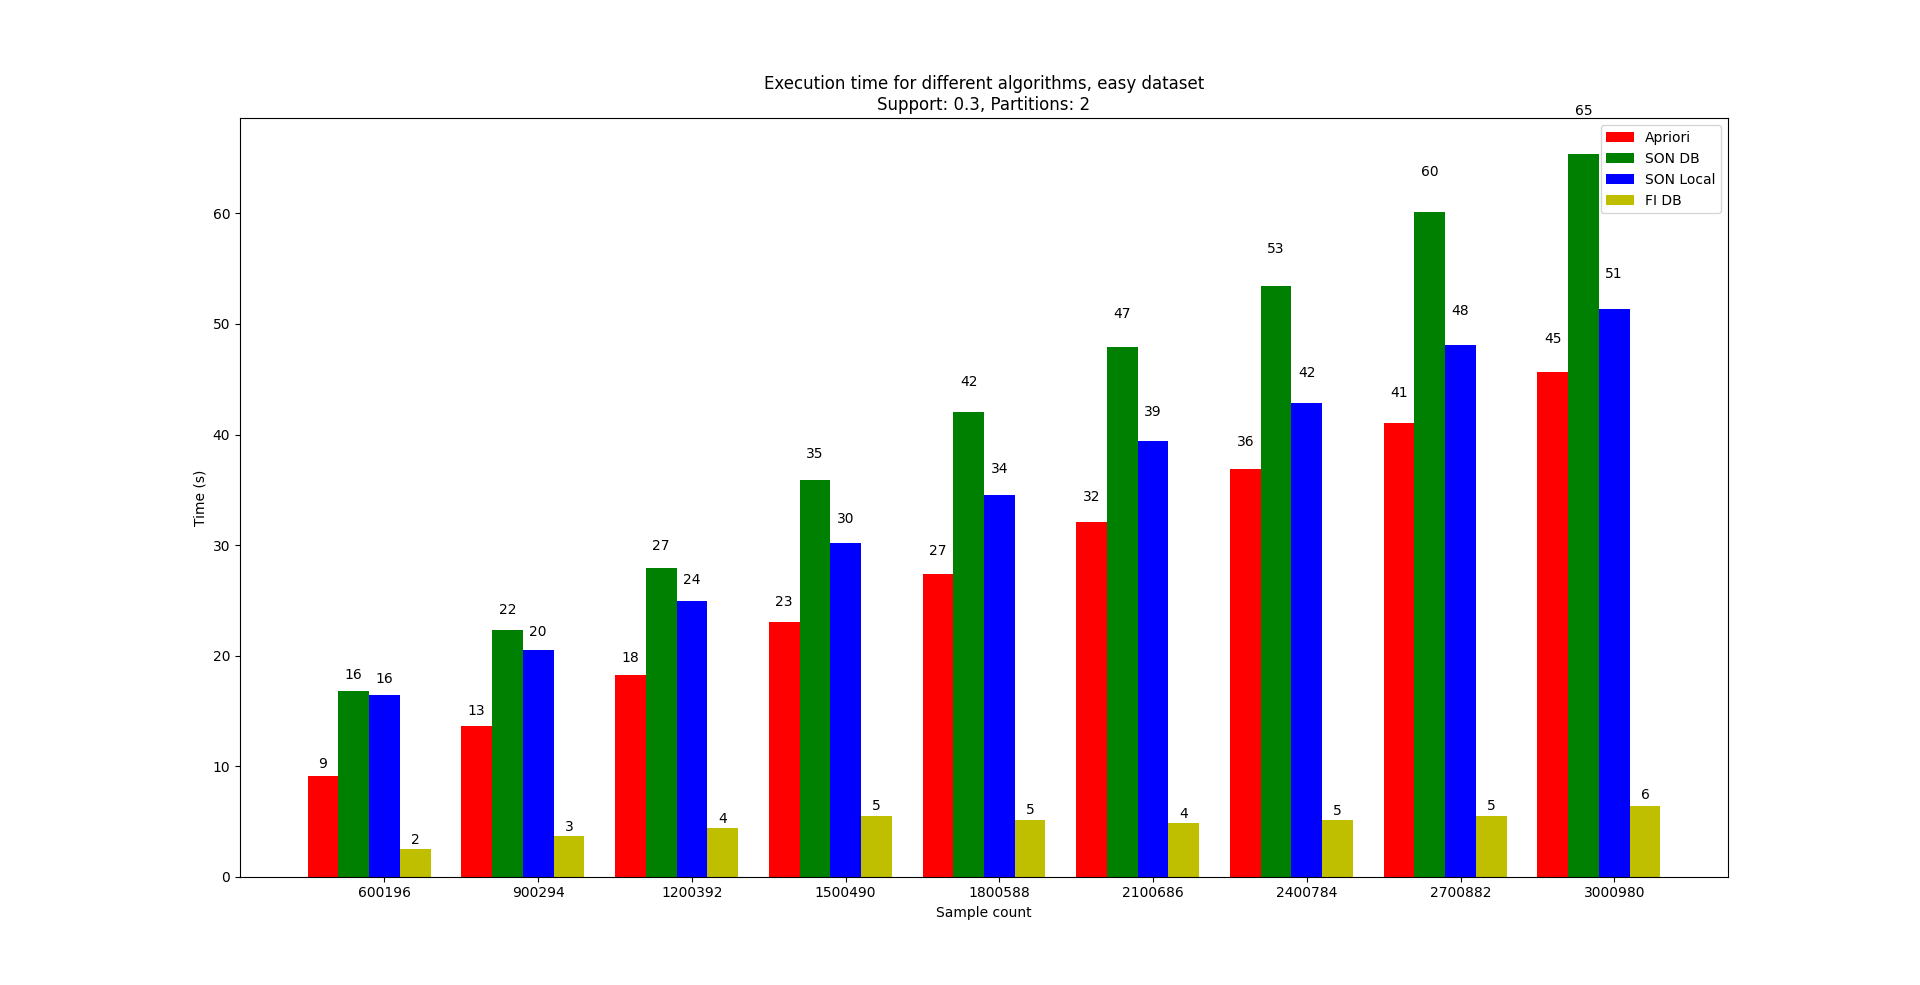
\includegraphics[width=\textwidth]{1_easy_0,3_2_dataset.png}
         	\caption{Easy dataset}
		\end{subfigure}
		\hfill		
		\begin{subfigure}[b]{\textwidth}
			\centering
			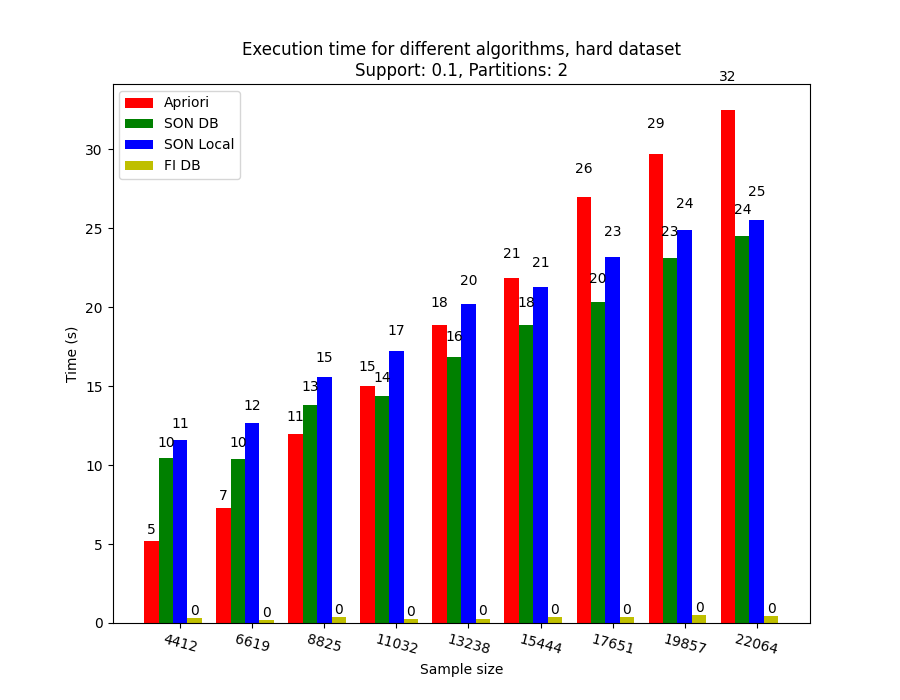
\includegraphics[width=\textwidth]{1_hard_0,1_2_dataset.png}
         	\caption{Hard dataset}
		\end{subfigure}
		\hfill

		\caption{Two partitions, minimum support benchmarks}
		\label{fig:2par-minsup}
		
	\end{figure}
	
	
	
	
	\begin{figure}[h]
		\centering
		\begin{subfigure}[b]{\textwidth}
			\centering
			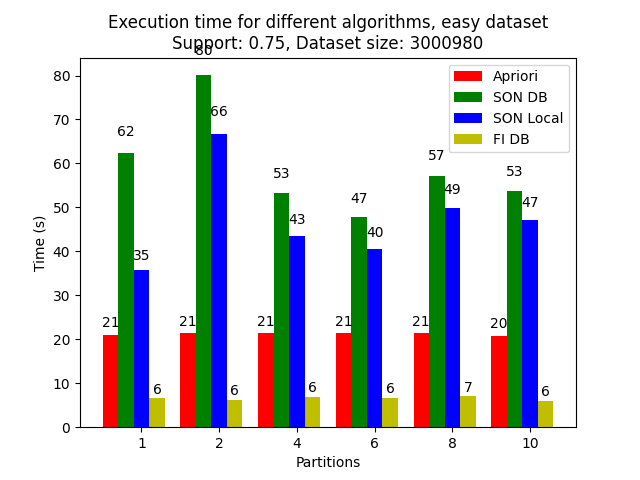
\includegraphics[width=\textwidth]{1_easy_0,75_1_partitions.png}
         	\caption{Easy dataset}
         	\label{fig:075sup-e}
		\end{subfigure}
		\hfill		
		\begin{subfigure}[b]{\textwidth}
			\centering
			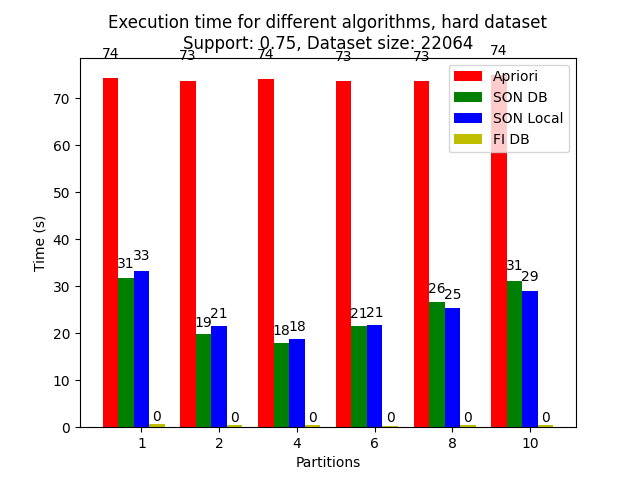
\includegraphics[width=\textwidth]{1_hard_0,75_1_partitions.png}
         	\caption{Hard dataset}
         	\label{fig:075sup-h}
		\end{subfigure}
		\hfill
		
		\caption{Partitions with 75\% support, full dataset}
		\label{fig:075sup}
	\end{figure}
	
	\begin{figure}[h]
		\centering
		\begin{subfigure}[b]{\textwidth}
			\centering
			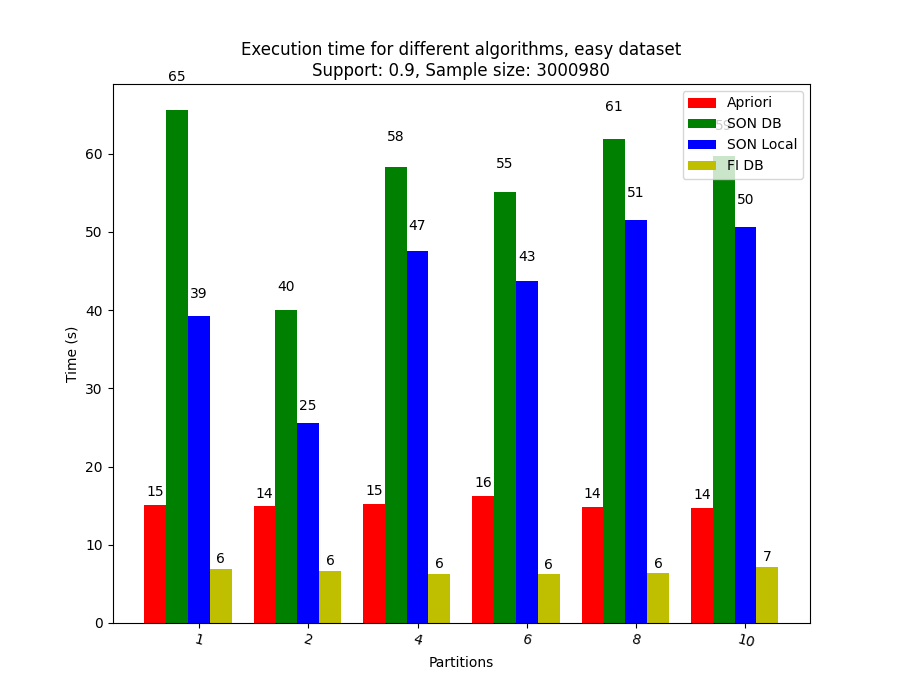
\includegraphics[width=\textwidth]{1_easy_0,9_1_partitions.png}
         	\caption{Easy dataset}
         	\label{fig:09sup-e}
		\end{subfigure}
		\hfill		
		\begin{subfigure}[b]{\textwidth}
			\centering
			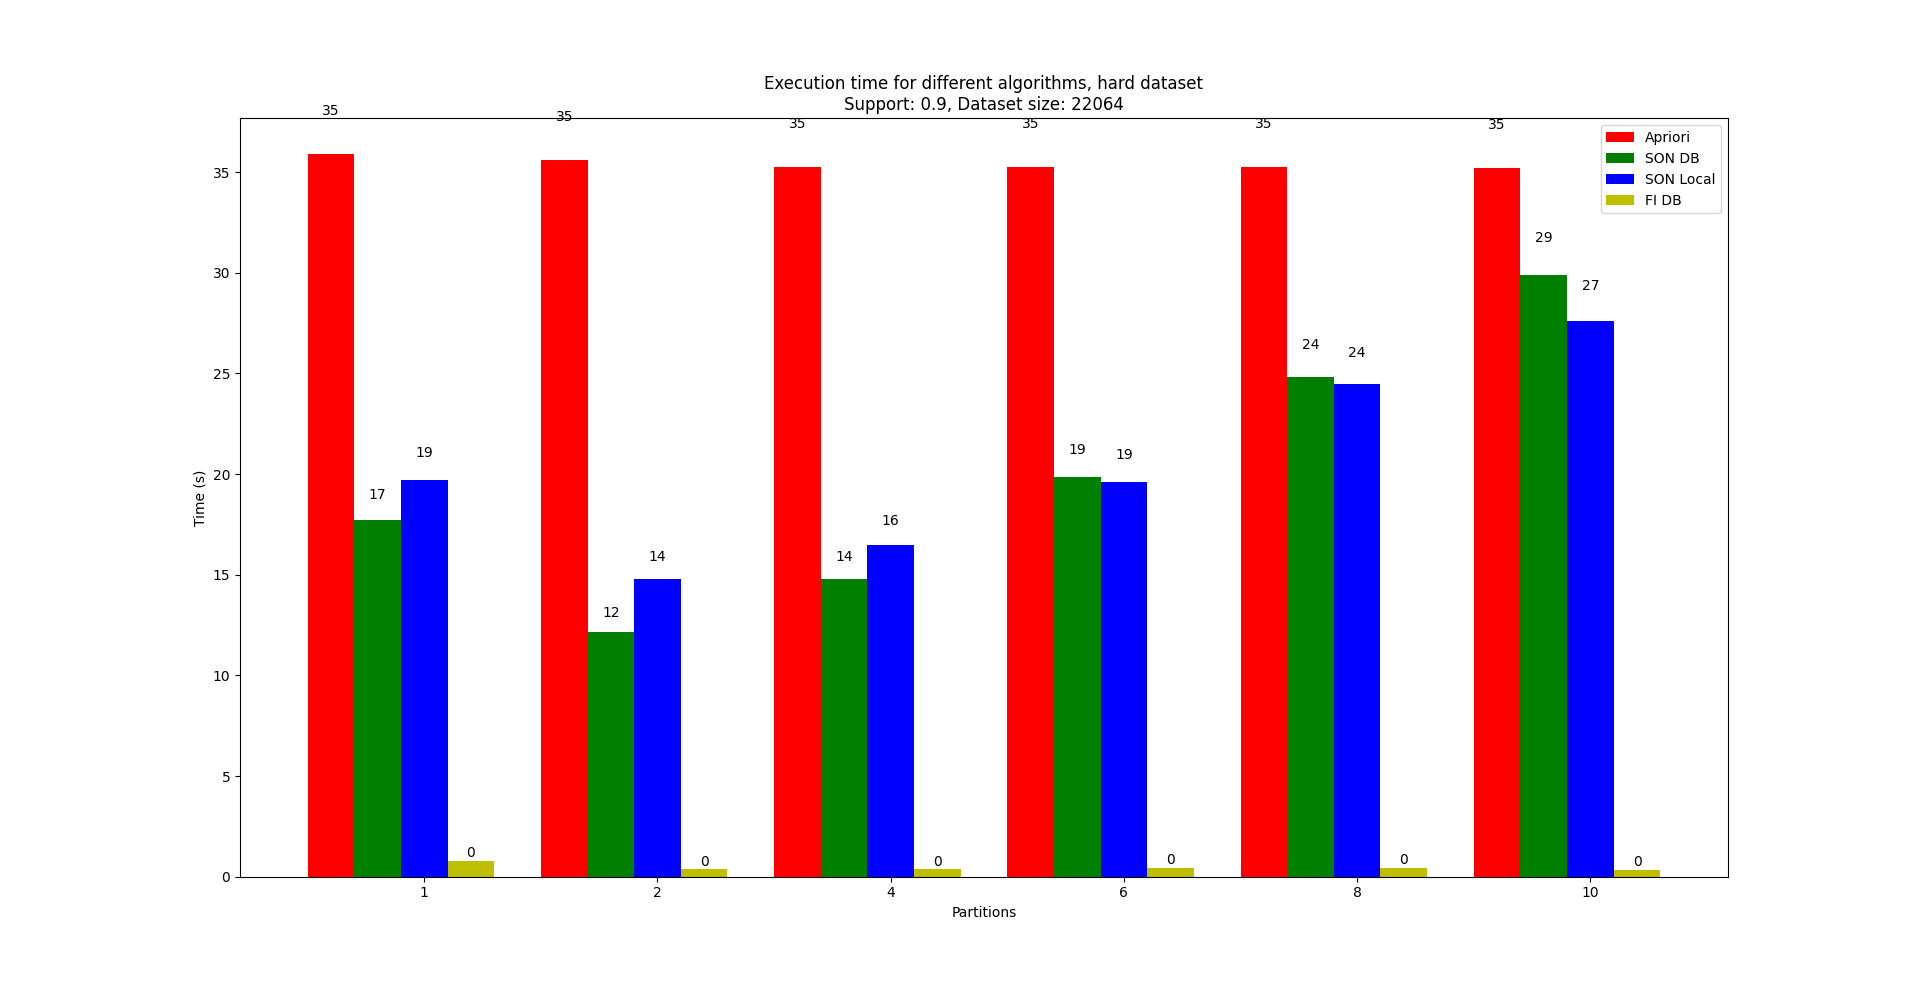
\includegraphics[width=\textwidth]{1_hard_0,9_1_partitions.png}
         	\caption{Hard dataset}
         	\label{fig:09sup-h}
		\end{subfigure}
		\hfill
		
		\caption{Partitions with 90\% support, full dataset}
		\label{fig:09sup}
	\end{figure}
\end{document}